\documentclass[]{article}
\usepackage[a4paper,top=3cm,bottom=2.5cm,left=2.5cm,
            right=2cm,marginparwidth=1.75cm,
            headheight=5pt]{geometry}
\usepackage[T5]{fontenc}
\usepackage[utf8]{inputenc}
\usepackage[document]{ragged2e}
\usepackage[vietnamese]{babel}
\usepackage[unicode]{hyperref}
\usepackage{amsmath}
\usepackage{setspace}
\usepackage{graphicx}
\usepackage{caption}
\usepackage{subcaption}
\usepackage{tcolorbox}
\usepackage{listings}
\usepackage{hyperref}
\usepackage{xcolor}
\usepackage{longtable}
\usepackage{titlesec}
\usepackage{floatrow}
\usepackage[nottoc]{tocbibind}
\usepackage{mdframed}
\usepackage{amsmath}
\usepackage{amssymb}
\usepackage{tgbonum}
\usepackage{type1cm}
\usepackage{indentfirst}
\usepackage{lettrine}
\usepackage{colortbl}
\usepackage{fancyhdr}
\usepackage{wrapfig}
\usepackage{lastpage}
\usepackage{url}
\addto\captionsenglish{
  \renewcommand{\contentsname}{MỤC LỤC}%
  \renewcommand{\listfigurename}{Danh sách ảnh}%
  \renewcommand{\listtablename}{Danh sách bảng}%
  \renewcommand{\figurename}{Hình}
  \renewcommand{\tablename}{Bảng}
}
\pagestyle{fancy}
\fancyhf{}
\rhead{Toán ứng dụng và thống kê}
\lhead{\color{cyan}Đồ án 2: Image Processing}
\lfoot{Trang \thepage /\pageref{LastPage}}
\renewcommand{\footrulewidth}{0.4pt}
\setlength{\parindent}{5pt}
\setlength{\parskip}{1cm}
\renewcommand{\baselinestretch}{1.5}
\newmdenv[linecolor=black,skipabove=\topsep,skipbelow=\topsep,
leftmargin=2.5cm,rightmargin=2.5cm,
innerleftmargin=5cm,innerrightmargin=5cm]{mybox}
\usepackage{multicol}
\usepackage{indentfirst}
\usepackage{color}
\usepackage{apacite}
\usepackage{tikz}
\graphicspath{{Figures/}} 
\usepackage[square, numbers, comma, sort&compress]{natbib}  
\usepackage{lipsum}
\usetikzlibrary{calc}
\setlength{\columnseprule}{2pt}
\def\columnseprulecolor{\color{black}}
\def\maru#1{\textcircled{\scriptsize#1}}

\begin{document}
% Bìa trang
\begin{titlepage}
\begin{tikzpicture}[remember picture,overlay,inner sep=0,outer sep=0]
     \draw[blue!70!black,line width=4pt] ([xshift=-1.5cm,yshift=-2cm]current page.north east) coordinate (A)--([xshift=2cm,yshift=-2cm]current page.north west) coordinate(B)--([xshift=2cm,yshift=2cm]current page.south west) coordinate (C)--([xshift=-1.5cm,yshift=2cm]current page.south east) coordinate(D)--cycle;

     \draw ([yshift=0.5cm,xshift=-0.5cm]A)-- ([yshift=0.5cm,xshift=0.5cm]B)--
     ([yshift=-0.5cm,xshift=0.5cm]B) --([yshift=-0.5cm,xshift=-0.5cm]B)--([yshift=0.5cm,xshift=-0.5cm]C)--([yshift=0.5cm,xshift=0.5cm]C)--([yshift=-0.5cm,xshift=0.5cm]C)-- ([yshift=-0.5cm,xshift=-0.5cm]D)--([yshift=0.5cm,xshift=-0.5cm]D)--([yshift=0.5cm,xshift=0.5cm]D)--([yshift=-0.5cm,xshift=0.5cm]A)--([yshift=-0.5cm,xshift=-0.5cm]A)--([yshift=0.5cm,xshift=-0.5cm]A);


     \draw ([yshift=-0.3cm,xshift=0.3cm]A)-- ([yshift=-0.3cm,xshift=-0.3cm]B)--
     ([yshift=0.3cm,xshift=-0.3cm]B) --([yshift=0.3cm,xshift=0.3cm]B)--([yshift=-0.3cm,xshift=0.3cm]C)--([yshift=-0.3cm,xshift=-0.3cm]C)--([yshift=0.3cm,xshift=-0.3cm]C)-- ([yshift=0.3cm,xshift=0.3cm]D)--([yshift=-0.3cm,xshift=0.3cm]D)--([yshift=-0.3cm,xshift=-0.3cm]D)--([yshift=0.3cm,xshift=-0.3cm]A)--([yshift=0.3cm,xshift=0.3cm]A)--([yshift=-0.3cm,xshift=0.3cm]A);

   \end{tikzpicture}
\newcommand{\HRule}{\rule{\linewidth}{0.5mm}}
\center

\textsc{\Large TRƯỜNG ĐẠI HỌC KHOA HỌC TỰ NHIÊN}\\[0.5cm]
\textsc{\Large KHOA CÔNG NGHỆ THÔNG TIN}\\[1cm]

\includegraphics[width=0.3\textwidth]{logo/KHTN.jpg}\\[1cm]

\HRule \\[0.4cm]
{\huge \bfseries ĐỒ ÁN 2: IMAGE PROCESSING} \\[0.4cm]
{\large TOÁN ỨNG DỤNG VÀ THỐNG KÊ}\\[0.1cm]
\HRule \\[1.5cm]

\centerline{\Large{\textbf{Triệu Nhật Minh — 21127112 — 21CLC02}}}
\vspace{2.5cm}
\centerline{\large{\textit{Giảng viên hướng dẫn}}}
\vspace{0.25cm}
\centerline{\large{Vũ Quốc Hoàng}}
\centerline{\large{Lê Thanh Tùng}}
\centerline{\large{Nguyễn Văn Quang Huy}}
\centerline{\large{Phan Thị Phương Uyên}}

\vspace{2.5cm}
\centerline{\today}


\vfill % Wipe blank space of the page.
\end{titlepage}

% Mục lục tự động
\setlength{\parskip}{.7em}
\tableofcontents
\newpage

% Table of Figures & Tables
\setlength{\parskip}{.5em}
%\listoffigures
%\listoftables
\newpage

% Bắt đầu nội dung
\section{Hướng dẫn sử dụng}
\begin{description}
  \item[Bước 1:] Run all các cell trong notebook \textbf{21127112.ipynb} (hoặc chỉ run cell cuối cùng để chạy hàm main nếu đã khởi chạy các hàm bổ trợ từ trước).
  \item[Bước 2: ] Nhập đường dẫn tới ảnh cần xử lý (chỉ cần tên ảnh nếu ảnh đã nằm cùng thư mục với notebook).
  \item[Bước 3: ] Chọn chức năng cần thực hiện (từ 0-8 tương ứng với các chức năng và 9 để thoát chương trình).
  \item[Bước 4: ] 
\end{description}

\section{Đánh giá kết quả}
\begin{longtable}[c]{|r|l|c|l|}
  \hline
  \rowcolor[HTML]{00D2CB} 
  \multicolumn{1}{|c|}{\cellcolor[HTML]{00D2CB}{\color[HTML]{FFFFFF} \textbf{STT}}} & \multicolumn{1}{c|}{\cellcolor[HTML]{00D2CB}{\color[HTML]{FFFFFF} \textbf{Chức năng}}} & {\color[HTML]{FFFFFF} \textbf{Mức độ hoàn thành}} & \multicolumn{1}{c|}{\cellcolor[HTML]{00D2CB}{\color[HTML]{FFFFFF} \textbf{Kết quả}}} \\ \hline
  \endfirsthead
  %
  \endhead
  1 & Thay đổi độ sáng cho ảnh & 100\% & \parbox[c]{8em}{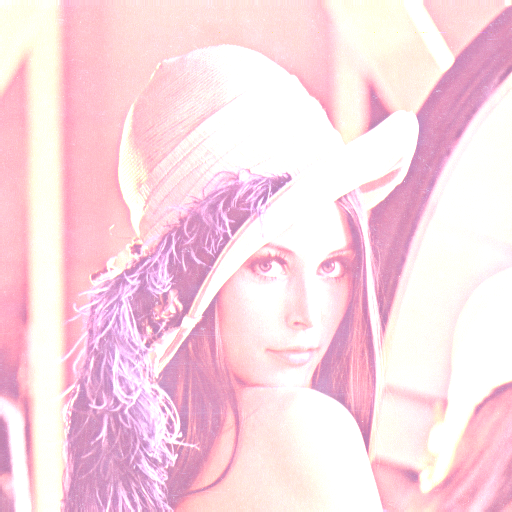
\includegraphics[width=8em]{image/Lenna_brightness_128.png}} \\ \hline
  2 & Thay đổi độ tương phản & 100\% & \parbox[c]{8em}{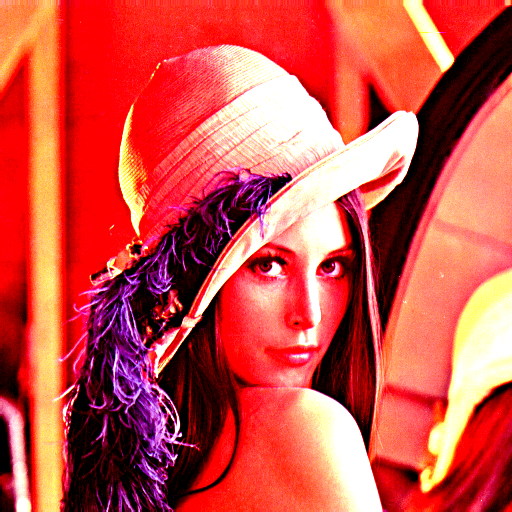
\includegraphics[width=8em]{image/Lenna_contrast_128.png}} \\ \hline
  3 & Lật ảnh ngang & 100\% & \parbox[c]{8em}{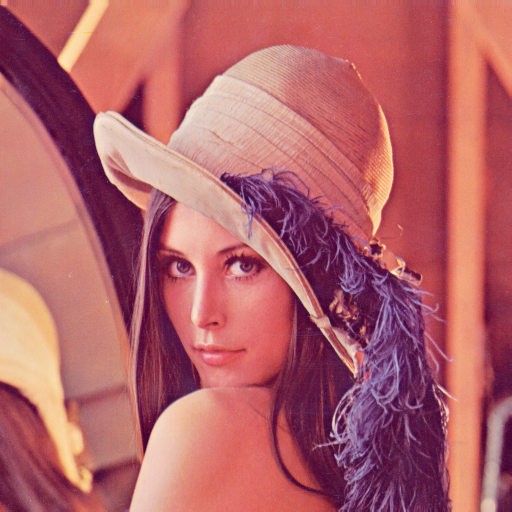
\includegraphics[width=8em]{image/Lenna_flip_horizontal.png}} \\ \hline
  4 & Lật ảnh dọc & 100\% & \parbox[c]{8em}{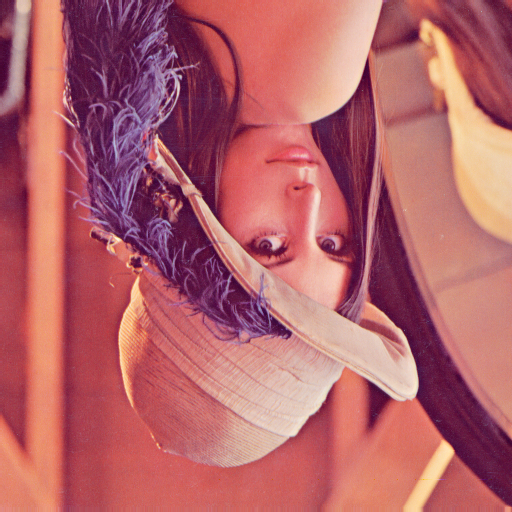
\includegraphics[width=8em]{image/Lenna_flip_vertical.png}} \\ \hline 
  5 & Chuyển đổi thành ảnh xám & 100\% & \parbox[c]{8em}{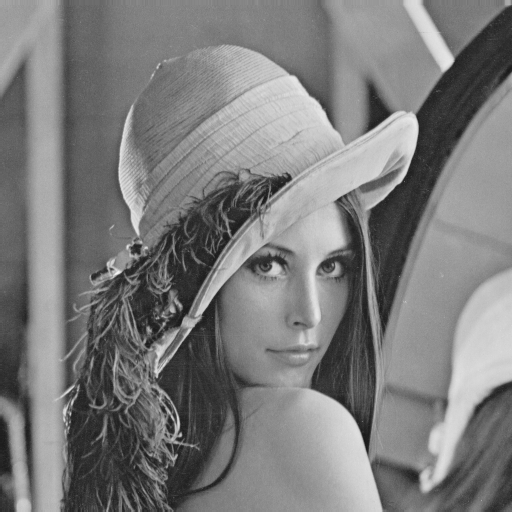
\includegraphics[width=8em]{image/Lenna_grayscale.png}} \\ \hline
  6 & Chuyển đổi thành ảnh sepia & 100\% & \parbox[c]{8em}{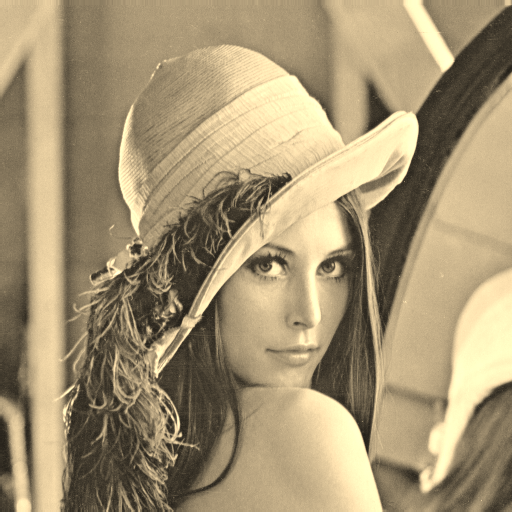
\includegraphics[width=8em]{image/Lenna_sepia.png}} \\ \hline
  7 & Làm mờ & 100\% & \parbox[c]{8em}{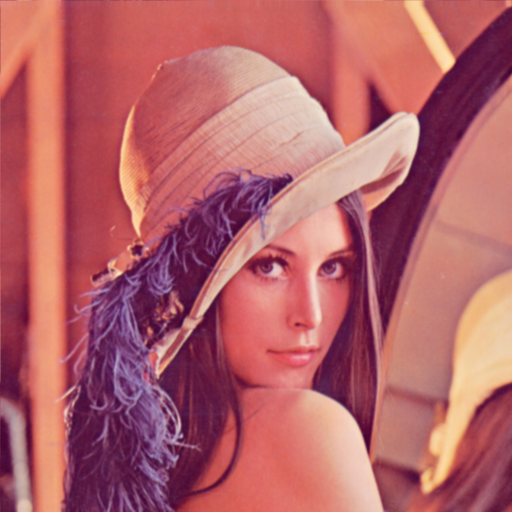
\includegraphics[width=8em]{image/Lenna_blur.png}} \\ \hline
  8 & Làm sắc nét ảnh & 100\% & \parbox[c]{8em}{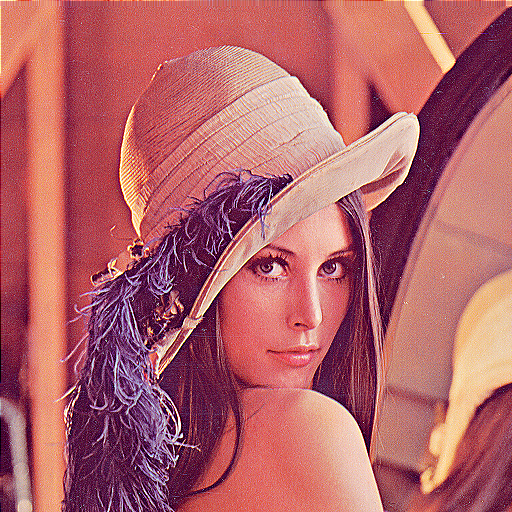
\includegraphics[width=8em]{image/Lenna_sharpen.png}} \\ \hline
  9 & Cắt ảnh theo kích thước (cắt ở trung tâm) & 100\% & \parbox[c]{8em}{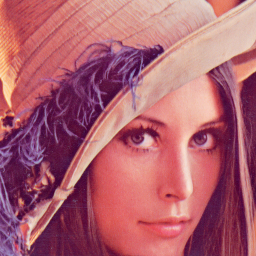
\includegraphics[width=8em]{image/Lenna_center_crop.png}} \\ \hline
  10 & Cắt ảnh theo khung hình tròn & 100\% & \parbox[c]{8em}{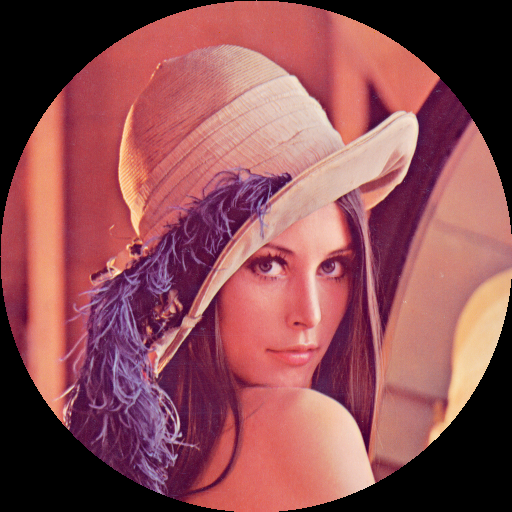
\includegraphics[width=8em]{image/Lenna_circular_crop.png}} \\ \hline
  11 & Cắt ảnh theo khung elip & 100\% & \parbox[c]{8em}{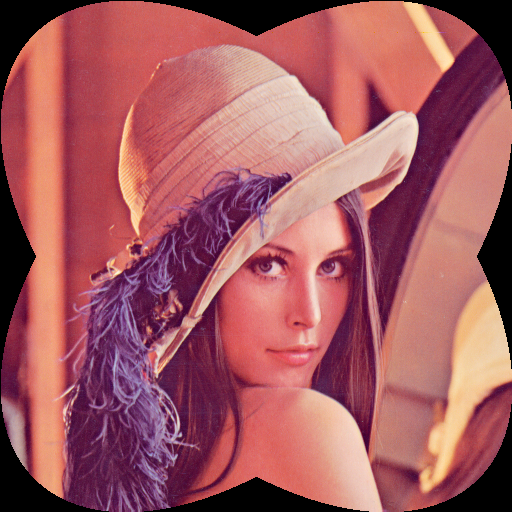
\includegraphics[width=8em]{image/Lenna_elliptical_crop.png}} \\ \hline
\end{longtable}

\section{Mô tả}
\textcolor{red}{Để thuận tiện cho phần trình bày bên dưới, từ bây giờ, mỗi điểm ảnh gồm 3 giá trị của kênh màu RGB sẽ được xem như một phần tử màu. Do đó, ma trận các điểm ảnh được xem như mảng 2 chiều các điểm ảnh, kí hiệu: \textit{img\_2d}. }
% Template mô tả hàm
% \textbf{Input:} \\
% \textbf{Output:}
% \paragraph{Ý tưởng thực hiện:}
% \paragraph{Mô tả:}
\subsection{Nhóm hàm chính}
\subsubsection{Hàm change\_brightness}
\textbf{Input:} Mảng NumPy 2 chiều các điểm ảnh \textit{img\_2d}, giá trị độ sáng \textit{brightness} (mặc định là 128 nếu không truyền tham số vào hàm). \\
\textbf{Output:} Mảng NumPy 2 chiều các điểm ảnh, chuỗi kí tự chứa hậu tố của tên file ảnh sau xử lý.

\paragraph{Ý tưởng thực hiện:} Thay đổi độ sáng bức ảnh là cùng lúc thay đổi giá trị trong phần tử màu của từng pixel ảnh cho một hằng số. \\
Xét một pixel ảnh $p$ thuộc hệ màu RGB, giá trị của từng kênh màu là $[p_{1}, p_{2}, p_{3}]$. Giá trị của pixel ảnh $p$ sau khi thay đổi độ sáng được tính bằng công thức: 
\[[p_{1} + k , p_{2} + k, p_{3} + k]\]
với $k$ là hằng số thay đổi độ sáng. \par Bức ảnh sau khi thay đổi độ sáng sẽ có màu sáng hơn hoặc tối hơn tùy thuộc vào giá trị của hằng số này, càng tối nghĩa là càng nhiều pixel có giá trị màu gần 0 và ngược lại.

\paragraph{Mô tả:} Để thay đổi độ sáng của ảnh, ta chỉ cần cộng thêm giá trị \textit{brightness} vào mỗi giá trị trong phần tử màu của mảng \textit{img\_2d}. Tuy nhiên, giá trị này có thể vượt quá khoảng giá trị cho phép của một giá trị của phần tử màu (từ 0 đến 255). Do đó, trước khi thực hiện phép cộng, ta cần đổi kiểu dữ liệu của mảng \textit{img\_2d} thành int64 để có thể lưu được các giá trị nguyên âm và giá trị nguyên dương lớn hơn 255. Sau khi thực hiện xong, kết hợp việc giới hạn giá trị sử dụng hàm \textit{limit\_value} và ép kiểu dữ liệu về uint8, ta được mảng 2 chiều các điểm ảnh sau khi thay đổi độ sáng. Việc ép kiểu mảng trước khi thực hiện phép cộng nhằm đảm bảo từng giá trị màu trong mỗi pixel không bị sai lệch giá trị (256 sẽ trở về 0 nếu không ép kiểu về int64).

\subsubsection{Hàm change\_contrast}
\textbf{Input:} Mảng NumPy 2 chiều các điểm ảnh \textit{img\_2d}, giá trị tương phản \textit{contrast} (mặc định là 128 nếu không truyền tham số vào hàm). \\
\textbf{Output:} Mảng NumPy 2 chiều các điểm ảnh, chuỗi kí tự chứa hậu tố của tên file ảnh sau xử lý.

\paragraph{Ý tưởng thực hiện:} Tương tự như việc thay đổi độ sáng của bức ảnh, thay đổi độ tương phản của bức ảnh là cùng lúc thay đổi giá trị trong phần tử màu của từng pixel ảnh cho một hằng số. Thay vì phép cộng như thay đổi độ sáng, giá trị của một phần tử màu thay đổi theo công thức:
\[ \text{R'} = \text{F} \times (\text{R}-128) + 128 \]
với:
\begin{itemize}
    \item \textit{R'} là giá trị của phần tử màu sau khi thay đổi độ tương phản.
    \item \textit{R} là giá trị của phần tử màu trước khi thay đổi độ tương phản.
    \item \textit{F} là hằng số thay đổi độ tương phản. Với \textit{C} là giá trị tương phản truyền vào hàm thì công thức của hằng số này:
    \[ \text{F} = \frac{259(\text{C}+255)}{255(259-\text{C})} \]
\end{itemize}

\paragraph{Mô tả:} Do \textit{F} được tính bởi công thức trên nên giá trị của \textit{F} có thể vượt quá 1, kéo theo đó, giá trị của mảng \textit{img\_2d} có thể vượt quá khoảng giá trị cho phép của một giá trị của phần tử màu (từ 0 đến 255). Do đó, trước khi thực hiện phép nhân, ta cần đổi kiểu dữ liệu của mảng \textit{img\_2d} thành float64 để có thể lưu được các giá trị số thực nhỏ hơn 0 và lớn hơn 255. Sau khi thực hiện xong, kết hợp việc giới hạn giá trị sử dụng hàm \textit{limit\_value} và ép kiểu dữ liệu về uint8, ta được mảng 2 chiều các điểm ảnh sau khi thay đổi độ tương phản.

\subsubsection{Hàm flip\_image}
\textbf{Input:} Mảng NumPy 2 chiều các điểm ảnh \textit{img\_2d}, hướng lật cần xử lý \textit{axis}. \\
\textbf{Output:} Mảng NumPy 2 chiều các điểm ảnh đã được lật theo hướng \textit{axis}, chuỗi kí tự chứa hậu tố của tên file ảnh sau xử lý.

\paragraph{Ý tưởng thực hiện:} Để lật ảnh theo chiều dọc, ta chỉ cần đảo ngược thứ tự các hàng của mảng \textit{img\_2d}, tương tự, để lật ảnh theo chiều ngang, ta chỉ cần đảo ngược thứ tự các cột của mảng. Để thực hiện được việc đảo ngược thứ tự các hàng hoặc cột của mảng mà không sử dụng hàm có sẵn của thư viện NumPy, ta sẽ sử dụng kỹ thuật slicing của Python.

\paragraph{Mô tả:} Trong hàm flip\_image, giá trị 0 và 1 được sử dụng để chỉ định trục mà hình ảnh sẽ được lật. Trong trường hợp này, giá trị 0 được sử dụng để chỉ định trục dọc (trục y) và giá trị 1 được sử dụng để chỉ định trục ngang (trục x), cách đánh số này phù hợp với cách đánh số các trục khi trục dọc được đánh số là trục thứ nhất và trục ngang được đánh số là trục thứ hai.
\begin{itemize}
  \item img\_2d[::-1, :]:
  Cú pháp này sẽ lấy toàn bộ các hàng của mảng \textit{img\_2d} nhưng đảo ngược thứ tự của chúng. Điều này có nghĩa là hàng đầu tiên sẽ trở thành hàng cuối cùng, hàng thứ hai sẽ trở thành hàng áp chót, và ngược lại. Kết quả thu được là một mảng mới với cùng kích thước như mảng ban đầu nhưng được lật theo chiều dọc.
  \item img\_2d[:, ::-1]:
  Cú pháp này sẽ lấy toàn bộ các cột của mảng \textit{img\_2d} nhưng đảo ngược thứ tự của chúng. Kết quả thu được là một mảng mới với cùng kích thước như mảng ban đầu nhưng được lật theo chiều ngang.
\end{itemize}
Dù lấy toàn bộ hàng hay cột của mảng thì phần tử màu của ảnh vẫn được giữ nguyên, chỉ thứ tự của chúng bị đảo ngược, do đó ở chiều thứ ba của mảng ảnh, ta không cần thực hiện việc slicing.

\subsubsection{Hàm convert\_grayscale}
\textbf{Input:} Mảng NumPy 2 chiều các điểm ảnh \textit{img\_2d}. \\
\textbf{Output:} Mảng NumPy 2 chiều các điểm ảnh đã được chuyển sang ảnh xám, chuỗi kí tự chứa hậu tố của tên file ảnh sau xử lý.

\paragraph{Ý tưởng thực hiện:} Để chuyển ảnh màu sang ảnh xám, ta sẽ sử dụng công thức sau (luminosity method):
\[ \text{Y} = 0.3*\text{R} + 0.59*\text{G} + 0.11*\text{B}\]
Trong đó, R, G, B lần lượt là giá trị của các phần tử màu Red, Green, Blue của điểm ảnh đang xét. Sau khi tính được giá trị Y, ta sẽ gán giá trị Y cho cả 3 phần tử màu của điểm ảnh đang xét. Và một cách dễ hình dung, ta nhân vô hướng vector [R, G, B] của từng điểm ảnh với vector [0.3, 0.59, 0.11] để tính được giá trị Y. Để thực hiện được việc nhân vô hướng này, ta sẽ sử dụng hàm dot của thư viện NumPy.

Cần lưu ý rằng tích vô hướng của 2 vector là một số (scalar), nhưng mỗi điểm ảnh trong bức ảnh cần 3 kênh màu (với hệ màu RGB), ta cần lặp lại giá trị Y 3 lần để gán cho điểm ảnh đang xét. Để thực hiện việc lặp lại này, ta sẽ sử dụng hàm repeat của thư viện NumPy theo trục cuối cùng (\textit{axis=-1}).

\paragraph{Mô tả:}
Đối với hàm NumPy dot \textcolor{red}{\textit{numpy.dot(a, b, out=None)}}, nếu a là mảng nhiều chiều và b là mảng một chiều thì kết quả là tích vô hướng trên trục cuối cùng của a và b. Tận dụng đặc tính này của hàm, ta sẽ nhân vô hướng mảng \textit{img\_2d} với mảng 1 chiều [0.3, 0.59, 0.11]. Do trục cuối cùng của mảng \textit{img\_2d} là mảng 1 chiều chứa giá trị của 3 phần tử màu của điểm ảnh, nên kết quả thu được là mảng 2 chiều chứa giá trị Y của các điểm ảnh (\textit{gray\_image}). 

Tham số cần truyền vào hàm repeat lần lượt là mảng chứa các giá trị cần lặp lại, số lần lặp lại (\textit{repeats}), và trục cần lặp lại (\textit{axis}). Mảng \textit{gray\_image} đang là mảng 2 chiều chứa giá trị Y của các điểm ảnh, ta sẽ mở rộng mảng này thêm 1 chiều ở trục cuối cùng bằng cách sử dụng \textit{gray\_image[...,None]}, sau đó lặp lại mảng này 3 lần (một cách tổng quát hơn là \textit{img\_2d.shape[-1]} lần) theo trục cuối cùng. Với công thức chuyển đổi ảnh xám sử dụng luminosity method như trên, giá trị Y đảm bảo hợp lệ nên ta không cần thực hiện việc giới hạn giá trị cũng như ép kiểu kết quả thu được.

\subsubsection{Hàm convert\_sepia}
\textbf{Input:} Mảng NumPy 2 chiều các điểm ảnh \textit{img\_2d}. \\
\textbf{Output:} Mảng NumPy 2 chiều các điểm ảnh đã được chuyển sang ảnh sepia, chuỗi kí tự chứa hậu tố của tên file ảnh sau xử lý.

\paragraph{Ý tưởng thực hiện:} Để chuyển ảnh màu sang ảnh sepia, ta sẽ sử dụng công thức sau:
\begin{align*}
  \text{newRed} = 0.393*\text{R} + 0.769*\text{G} + 0.189*\text{B} \\
  \text{newGreen} = 0.349*\text{R} + 0.686*\text{G} + 0.168*\text{B} \\
  \text{newBlue} = 0.272*\text{R} + 0.534*\text{G} + 0.131*\text{B} 
\end{align*}
với R, G, B lần lượt là giá trị của các phần tử màu Red, Green, Blue của điểm ảnh đang xét. Sau khi tính được giá trị newRed, newGreen, newBlue, ta lần lượt gán các giá trị trên vào các điểm ảnh. \\
Xét một pixel ảnh $p$ thuộc hệ màu RGB, giá trị của từng kênh màu là $[p_{1}, p_{2}, p_{3}]$. Ta có thể viết lại công thức trên dưới dạng ma trận như sau:
\begin{align*}
  \begin{bmatrix}
    \text{newRed} \\
    \text{newGreen} \\
    \text{newBlue}
  \end{bmatrix}
  =
  \begin{bmatrix}
    0.393 & 0.769 & 0.189 \\
    0.349 & 0.686 & 0.168 \\
    0.272 & 0.534 & 0.131
  \end{bmatrix}
  \begin{bmatrix}
    p_{1} \\
    p_{2} \\
    p_{3}
  \end{bmatrix}
\end{align*}
$\Leftrightarrow$
\begin{align*}
  \begin{bmatrix}
    \text{newRed} & \text{newGreen} & \text{newBlue}
  \end{bmatrix}
  =
  \begin{bmatrix}
    p_{1} & p_{2} & p_{3}
  \end{bmatrix}
  \begin{bmatrix}
    0.393 & 0.769 & 0.189 \\
    0.349 & 0.686 & 0.168 \\
    0.272 & 0.534 & 0.131
  \end{bmatrix}^\top
\end{align*}
Bằng việc ma trận hoá công thức trên, ta dễ dàng sử dụng hàm dot trong thư viện NumPy để thực hiện tính toán. Cần lưu ý rằng với trọng số như trên, các giá trị của phần tử màu có thể vượt quá giá trị cho phép của kiểu dữ liệu uint8 nên cần giới hạn giá trị của kết quả trả về.

\paragraph{Mô tả:}
Đối với hàm \textcolor{red}{np.dot(a, b, out=None)}, nếu a là một mảng nhiều chiều và b là một mảng hai chiều thì kết quả là tích vô hướng trên từng phần tử trên trục cuối cùng của a với trục gần cuối của b.\\
Do trục cuối cùng của mảng \textit{img\_2d} là mảng 1 chiều chứa 3 phần tử màu của điểm ảnh và trục gần cuối của ma trận chuyển vị của mảng \textit{sepia\_array} có giá trị là các hàng của mảng \textit{sepia\_array.T}, là trọng số của các kênh màu Red, Green, Blue trong công thức chuyển đổi ảnh màu sang ảnh sepia, nên kết quả của phép nhân này chính là giá trị của các kênh màu mới của điểm ảnh. \par
Với trọng số như trên, các giá trị của phần tử màu có thể vượt quá giá trị cho phép của kiểu dữ liệu uint8 nên cần giới hạn giá trị của kết quả trả về bằng hàm \textit{limit\_value}.

\subsubsection{Hàm convolute\_2D}
\textbf{Input:} Mảng NumPy 2 chiều các điểm ảnh \textit{img\_2d}, ma trận lọc \textit{kernel}. \\
\textbf{Output:} Kết quả của phép ''tích chập'' giữa NumPy 2 chiều các điểm ảnh \textit{img\_2d} với ma trận lọc \textit{kernel}, chuỗi kí tự chứa hậu tố của tên file ảnh sau xử lý. \\
\paragraph{Ý tưởng thực hiện:} Trong lĩnh vực xử lý ảnh, một kernel là một công cụ toán học được áp dụng lên ảnh để thực hiện các hiệu ứng như làm mờ, làm sắc nét, phát hiện cạnh,\dots Điều này được thực hiện bằng cách tính toán giá trị của mỗi pixel trong ảnh đầu ra dựa trên giá trị của các pixel xung quanh (bao gồm cả chính nó) trong ảnh đầu vào, kernel là ma trận chứa các hệ số để tính toán. \par
Về mặt toán học, công thức của phép tích chập (convolution) trong xử lý ảnh là:
\[ g(x, y) = \omega * f(x, y) = \sum_{dx=-a}^{a} \sum_{dy=-b}^{b} \omega (dx, dy) * f(x-dx, y-dy) \]
với:
\begin{itemize}
  \item $g(x, y)$ là giá trị của điểm ảnh ở vị trí $(x, y)$ trong ảnh đầu ra.
  \item $f(x, y)$ là giá trị của điểm ảnh ở vị trí $(x, y)$ trong ảnh đầu vào.
  \item $\omega$ là ma trận lọc (kernel).
  \item Mỗi phần tử của kernel bộ lọc nằm trong khoảng $-a \leq dx \leq a$ và $-b \leq dy \leq b$.
\end{itemize}

Nói về phép tích chập, tích chập là quá trình cộng từng phần tử của hình ảnh với các hàng xóm cục bộ của nó, có trọng số bởi kernel. Điều này liên quan đến một dạng tích chập toán học. Phép toán ma trận được thực hiện - tích chập - không phải là phép nhân ma trận. Gốc (origin) là vị trí của pixel đầu ra. Đối với một kernel đối xứng, gốc thường là phần tử ở trung tâm ma trận. \par 

Để tránh đi chi tiết về phép tích chập, phép tích chập được sử dụng trong hàm này là discrete convolution. Nếu thực hiện theo phương pháp tường minh, độ phức tạp của thuật toán này có thể lên đến $N^2$ với $N$ là kích thước của ma trận ảnh đầu vào. Tuy nhiên, ta có thể tối ưu bằng cách dùng thuật toán biến đổi Fourier nhanh (Fast Fourier Transform - FFT). Và trong NumPy có hàm \textit{numpy.fft.fftn} để thực hiện việc này. \par

Dù đã được tối ưu hơn nhưng phép tích chập mà ta nói đến từ đầu chỉ đang thực hiện trên mảng 2 chiều, nhưng với bức ảnh đầu ra là mảng 3 chiều, ta cần thực hiện phép tích chập trên từng kênh màu của ảnh đầu vào. 

Kernel được sử dụng trong hàm này là kernel Gaussian kích thước 3$\times$3 và kernel làm sắc nét kích thước 3$\times$3. Ma trận biểu diễn 2 kernel này được thể hiện như sau:
\[ \text{Gaussian kernel} = \frac{1}{16} \begin{bmatrix} 1 & 2 & 1 \\ 2 & 4 & 2 \\ 1 & 2 & 1 \end{bmatrix} \]
\[ \text{Sharpen kernel} = \begin{bmatrix} 0 & -1 & 0 \\ -1 & 5 & -1 \\ 0 & -1 & 0 \end{bmatrix} \]
\paragraph{Mô tả:} 
Nhằm phục vụ cho việc thực hiện tính chập nhanh dụng kỹ thuật FFT như đã nói ở trên, ta cần chuyển ma trận ảnh đầu vào và kernel về dạng ma trận phổ (spectrum) bằng cách sử dụng hàm \textit{numpy.fft.fftn} (\textcolor{red}{numpy.fft.fftn(a, s=None, axes=None)}). Sau đó, ta nhân 2 ma trận phổ này với nhau, và sử dụng hàm \textit{numpy.fft.ifftn} để chuyển về dạng ma trận điểm ảnh. \par

% Đoạn này dùng lúc sau khi giải thích dùng real


Tham số s trong hàm \textit{numpy.fft.fftn} xác định kích thước của mảng đầu ra. Trong trường hợp của hàm convolute\_2D, giá trị của tham số s được đặt là \textit{img\_2d.shape[:2]}. \par 

Khi sử dụng slicing [ :2], ta chỉ lấy hai phần tử đầu tiên của tuple này, làm cho kích thước của mảng đầu ra sẽ bằng với kích thước của hai chiều đầu tiên của mảng img\_2d. \par

Trong trường hợp cụ thể của kernel, điều này có nghĩa là kích thước của kernel\_fft sẽ bằng với kích thước của hai chiều đầu tiên của mảng img\_2d. Điều này giúp đảm bảo rằng kích thước của kernel\_fft và img\_fft (FFT của mảng 2 chiều các điểm ảnh) bằng nhau, do đó chúng có thể được nhân từng phần tử với nhau trong miền tần số bằng phép nhân element-wise. \par

Tham số axes trong hàm \textit{np.fft.fftn} xác định các trục mà phép biến đổi Fourier nhanh (FFT) được thực hiện. Bằng việc truyền tham sô \textit{axes=(0, 1)}, ta đang chỉ định rằng phép biến đổi FFT sẽ được thực hiện trên hai trục đầu tiên của mảng đầu vào. Với \textit{kernel}, phép biến đổi FFT sẽ được thực hiện trên toàn bộ kernel. Còn với mảng \textit{img\_2d}, mảng đầu vào là một mảng 3 chiều với kích thước (height, width, channels). Khi đặt axes=(0, 1), phép biến đổi FFT sẽ được thực hiện riêng biệt cho từng kênh màu của hình ảnh. Điều này được thực hiện bằng cách lặp qua từng kênh màu và tính FFT cho từng kênh một cách riêng biệt. \par

Với số lần lặp là không đáng kể (lặp với số kênh màu của bức ảnh), ta có thể dùng vòng lặp lần lượt thực hiện FFT trên từng kênh màu. FFT nghịch đảo là một phép biến đổi ngược lại của FFT, cho phép chuyển đổi một tín hiệu từ miền tần số về miền không gian. Trong trường hợp này, convolved\_fft là một tín hiệu trong miền tần số, do đó việc tính FFT nghịch đảo của nó sẽ cho ta kết quả trong miền không gian.

Sau khi tính FFT nghịch đảo, ta chỉ lấy phần thực của kết quả bằng cách sử dụng thuộc tính .real. Điều này là cần thiết vì kết quả của phép tính FFT nghịch đảo là một số phức, và ta chỉ quan tâm đến phần thực của nó. \par

Về phần \textcolor{blue}{padding}, từ hình minh hoạ:
\begin{figure}[!ht]
  \centering
  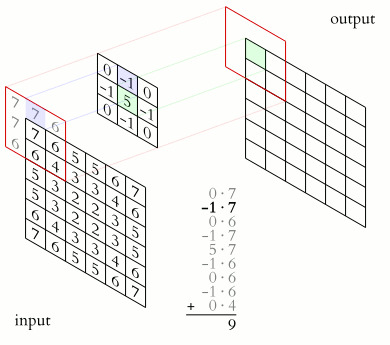
\includegraphics[width = 0.5\textwidth]{image/padding.jpg}
\end{figure}
\par

Với các điểm ảnh tại góc, ta có thể thấy rằng các điểm ảnh này không được tính toán với các điểm ảnh xung quanh, và để tránh kết quả không mong muốn khi tính toán, ta gọi hàm \textit{np.pad} để thêm các điểm ảnh ở xung quanh vào. \textit{numpy.pad} cho phép ta lựa chọn các điểm ảnh được thêm vào, và trong trường hợp này, ta thêm các điểm ảnh có giá trị bằng giá trị ở viền (edge) của ảnh. Với tham số \textit{pad\_width}, từ ảnh minh hoạ, ta có thể thấy rằng với kích thước kernel là 3x3 thì ta cần thêm (3 // 2 = 1) điểm ảnh vào ở mỗi cạnh của ảnh. Việc cắt padding [padding:-padding, padding:-padding] để loại bỏ các phần đệm của mảng kết quả sau khi tính FFT nghịch đảo. Ví dụ, với padding có giá trị là 1, thì slicing `[1:-1, 1:-1]` sẽ loại bỏ một hàng và một cột ở mép trên và mép dưới của mảng kết quả. Điều này giúp thu được một mảng mới có kích thước bằng với kích thước ban đầu của hình ảnh và không có các phần đệm.\par

Thực nghiệm cho thấy kết quả trả về của \textit{kernel\_fft} có kiểu dữ liệu của phần thực của phần tử là float64. Do đó, ta cần ép kiểu dữ liệu của mảng kết quả là float64 để tránh lỗi về kiểu dữ liệu. Kết quả cuối cùng trước khi thoát hàm cần được xử lý bởi hàm \textit{limit\_value} và được chuyển về kiểu dữ liệu uint8. \par


\subsubsection{Hàm blur\_image / sharpen\_image}
\textbf{Input:} Mảng NumPy 2 chiều các điểm ảnh \textit{img\_2d} \\
\textbf{Output:} Mảng NumPy 2 chiều các điểm ảnh \textit{img\_2d} đã được xử lý làm mờ hoặc sắc nét, chuỗi kí tự chứa hậu tố của tên file ảnh đầu ra. \\
\paragraph{Ý tưởng thực hiện:} Để làm mờ ảnh, ta cần thực hiện phép tích chập giữa ảnh đầu vào và kernel. Với kernel có kích thước 3x3, ta có thể thực hiện phép tích chập bằng cách gọi lại hàm \textit{convolve\_2d} đã được viết ở trên. Kernel được sử dụng là giá trị cố định được lưu trong biến \textit{gaussian\_kernel}. Tương tự, việc làm sắc nét cũng được thực hiện bằng cách gọi lại hàm \textit{convolve\_2d} với kernel là \textit{sharpen\_kernel}. \par
\paragraph{Mô tả:}
Về bản chất, việc gọi hai hàm này để truyền tham số là kernel và thực hiện tích chập cũng như tránh việc gọi hai hàm blur và sharpen cùng thực hiện tích chập với kernel khác nhau. Điều này giúp tổng thể đoạn code không bị lặp lại nhiều lần, thuận tiện cho việc tối ưu nếu có thể. \par

\subsubsection{Hàm center\_crop}
\textbf{Input:} Mảng NumPy 2 chiều các điểm ảnh \textit{img\_2d}, kích thước chiều cao \textit{height} và chiều rộng \textit{width} của ảnh đầu ra (mặc định kích thước ảnh đầu ra là 256x256 nếu ta không truyền 2 tham số này vào hàm). \\
\textbf{Output:} Mảng NumPy 2 chiều các điểm ảnh \textit{img\_2d} đã được cắt trung tâm theo kích thước \textit{height} và \textit{width}, và chuỗi kí tự chứa hậu tố của tên file ảnh đầu ra. \\
\paragraph{Ý tưởng thực hiện:} Với yêu cầu cắt ảnh từ trung tâm, ta cần xác định vị trí của pixel đầu tiên của ảnh đầu ra. Toạ độ của pixel đầu tiên của ảnh đầu ra (tạm gọi (\text{x\_{start}}, \text{y\_{start}})) được thể hiện như trên hình:
\begin{figure}[!ht]
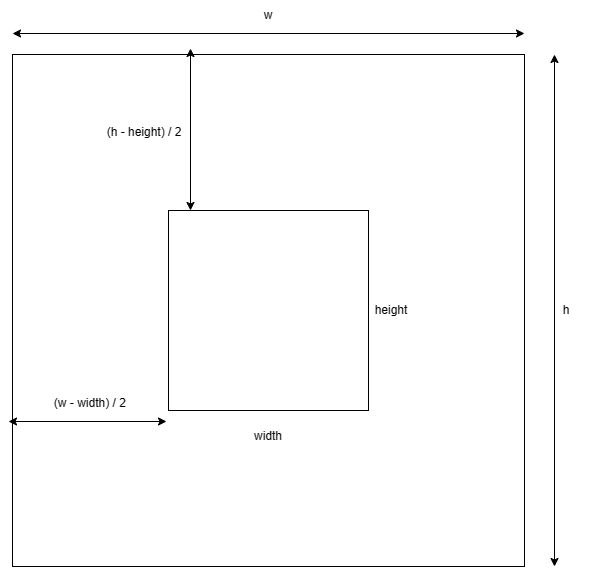
\includegraphics[width = .5\textwidth]{image/square_center.png}
\end{figure} \\
Từ vị trí \text{x\_{start}}, \text{y\_{start}} trên, ta có thể xác định vị trí của pixel cuối cùng của ảnh đầu ra (tạm gọi (\text{x\_{end}}, \text{y\_{end}})) như sau:
\begin{align*}
  \begin{cases}
    \text{x\_{end}} = \text{x\_{start}} + \text{height} \\
    \text{y\_{end}} = \text{y\_{start}} + \text{width}
  \end{cases}
\end{align*}
Với \textit{height} và \textit{width} là kích thước của ảnh đầu ra. \\
Sau khi xác định được vị trí của pixel đầu tiên và pixel cuối cùng của ảnh đầu ra, ta có thể cắt ảnh đầu vào theo vị trí này để được ảnh đầu ra bằng kỹ thuật slicing. 

\paragraph{Mô tả:} Ảnh đầu ra cần có kích thước \textit{height} x \textit{width} tính từ trung tâm bức ảnh  nên ta cần xác định vị trí của pixel đầu tiên của ảnh đầu ra. Từ phần ý tưởng ta có thể thấy toạ độ \text{x\_{start}}, \text{y\_{start}} được tính như trên hình và được thể hiện trong phần code, chỉ có điều để đảm bảo tính hợp lệ về kiểu dữ liệu cho mục đích slicing, phép chia lấy số nguyên (//) được sử dụng. Sau đó, bằng kỹ thuật slicing, ta cắt phần mảng từ y\_start đến y\_start + height theo chiều dọc và từ x\_start đến x\_start + width theo chiều ngang.

\subsubsection{Hàm circular\_crop}
\textbf{Input:} Mảng NumPy 2 chiều các điểm ảnh \textit{img\_2d} \\
\textbf{Output:} Mảng NumPy 2 chiều các điểm ảnh, với các pixel nằm ngoài hình tròn có bán kính định trước được gán giá trị 0 (màu đen), chuỗi kí tự chứa hậu tố của tên file ảnh đầu ra.
\paragraph{Ý tưởng thực hiện:} Đầu tiên, ta cần xác định tâm và bán kính của hình tròn cần cắt. Tâm của hình tròn được xác định bằng cách lấy trung bình của 2 giá trị \textit{height} và \textit{width} của ảnh đầu vào. Bán kính đường tròn nội tiếp hình vuông bằng một nửa chiều dài cạnh. Hình tròn bao gồm đường tròn và tất cả những điểm bên trong. Về mặt toán học, ta có thể biểu diễn hình tròn dưới dạng:
\[ (\text{x} - \text{x}\textsubscript 0)^2 + (\text{y} - \text{y}\textsubscript 0)^2 \leq \text{R}^2\]
với: 
\begin{itemize}
  \item \text{x}, \text{y} là tọa độ của một điểm bất kỳ đang xét
  \item \text{x}\textsubscript 0, \text{y}\textsubscript 0 là tọa độ của tâm hình tròn
  \item \text{R} là bán kính của đường tròn
\end{itemize}
Sau đó, tạo ra một mặt nạ mask để xác định các phần tử nằm ngoài vòng tròn cần cắt và gán giá trị của các phần tử nằm ngoài hình tròn bằng 0.
\paragraph{Mô tả:} Đầu tiên ta tìm toạ độ vị trí trung tâm của hình tròn cần cắt và bán kính hình tròn. Cách tính hai đại lượng đã được đề cập ở phần ý tưởng. Một cách ''tổng quát'' hơn để tìm bán kính là giá trị nhỏ hơn giữa $\frac{\textit{width}}{2}$ và $\frac{\textit{height}}{2}$. Việc chia lấy nguyên (//) được sử dụng để đảm bảo tính hợp lệ về kiểu dữ liệu phục vụ việc tạo mask.

Hàm NumPy ogrid trả về một lưới đa chiều (mảng) các giá trị tọa độ. Trong trường hợp này, ta sử dụng ogrid để tạo ra một mảng 2 chiều có kích thước bằng kích thước của ảnh đầu vào, trong đó mỗi phần tử là một tuple chứa 2 giá trị tọa độ. Sau đó, ta tính khoảng cách từ mỗi điểm ảnh đến tâm hình tròn và so sánh với bán kính hình tròn. Nếu điểm ảnh nằm trong đường tròn, giá trị mask tại điểm ảnh đó được gán bằng 0, ngược lại giá trị mask tại điểm ảnh đó được gán bằng 1. Dòng \textit{new\_img\_2d[mask] = 0} sử dụng mặt nạ mask để lựa chọn các phần tử nằm ngoài vòng tròn cần cắt trong mảng \textit{new\_img\_2d}, và đặt giá trị của chúng bằng 0. Điều này có nghĩa là các phần tử nằm trong vòng tròn cần cắt sẽ giữ nguyên giá trị, trong khi các phần tử nằm ngoài vòng tròn sẽ có giá trị mới bằng 0.

Ta hoàn toàn có thể không sử dụng bản sao của mảng \textit{img\_2d} và thay đổi trực tiếp giá trị trên chúng. Tuy nhiên, điều này sẽ làm thay đổi giá trị của mảng do Python luôn truyền tham chiếu khi truyền mảng vào hàm. Điều này có thể ảnh hưởng đến các tính toán sau này.

\subsubsection{Hàm elliptical\_crop}
\textbf{Input:} Mảng NumPy 2 chiều các điểm ảnh \textit{img\_2d} \\
\textbf{Output:} Mảng NumPy 2 chiều các điểm ảnh \textit{new\_img\_2d} đã được cắt theo hình elip, chuỗi kí tự chứa hậu tố của tên file ảnh đầu ra.
\paragraph{Ý tưởng thực hiện:} Phương trình elip được học ở chương trình phổ thông cho elip vuông góc với trục hoành hoặc trục tung. Tuy nhiên, khung ảnh elip xiên một góc nhất định, ta cần mở rộng công thức được học hơn:
\[ \frac{((x-x_0)\cos \alpha + (y-y_0) \sin \alpha)^2}{a^2} + \frac{((x-x_0)\sin \alpha - (y-y_0) \cos \alpha)^2}{b^2}= 1 \]
với:
\begin{itemize}
  \item \text{x}, \text{y} là tọa độ của một điểm bất kỳ đang xét
  \item \text{x}\textsubscript 0, \text{y}\textsubscript 0 là tọa độ của tâm hình elip
  \item \text{a}, \text{b} là độ dài trục lớn, trục nhỏ của hình elip. Trục lớn và trục nhỏ của elip vuông góc với nhau và chia elip thành hai nửa đối xứng.
  \item $\alpha$ là góc tạo bởi trục lớn hình elip và trục hoành của hệ trục toạ độ Oxy.
\end{itemize}
Để đảm bảo tính đối xứng qua các trục, nói cách khác, để đường chéo hình vuông là trục đối xứng của hình elip, ta chọn góc $\alpha$ là 45 độ hoặc 135 độ. Điều này giúp ta loại bỏ việc truyền góc $\alpha$ vào hàm, ta tính trực tiếp các giá trị $\cos \alpha$ và $\sin \alpha$ và thay vào phương trình, ta được:
\begin{equation}
  (\frac{1}{a^2} + \frac{1}{b^2})((x-x_0)^2 + (y-y_0)^2) \pm 2(\frac{1}{a^2} - \frac{1}{b^2})(x-x_0) (y-y_0) = 2
  \label{eq:elip}
\end{equation}
Tương tự như hàm \textit{circular\_crop}, ta sử dụng hàm \textit{numpy.ogrid} để tạo ra mask, tuy nhiên, ở khung ảnh elip này là 2 hình elip nên cần 2 mask. Bất kì điểm ảnh nào nằm ngoài cả 2 mask đều gán giá trị bằng 0. \par
Đến với việc tìm a, b cho phương trình elip, ta sẽ xem bức ảnh đầu vào có kích thước side$\times$side pixel. Để đơn giản, ta sẽ thu nhỏ tỉ lệ lại thành hình vuông kích thước 1$\times$1. Sử dụng phần mềm phác thảo hình học GeoGebra, để tối giản hai thành phần x\textsubscript 0, y\textsubscript 0, ta chọn hình vuông có toạ độ góc trái trên là (-0.5, 0.5) và góc phải dưới là (0,5, -0.5), minh hoạ như hình bên dưới:
\begin{figure}[!ht]
  \centering
  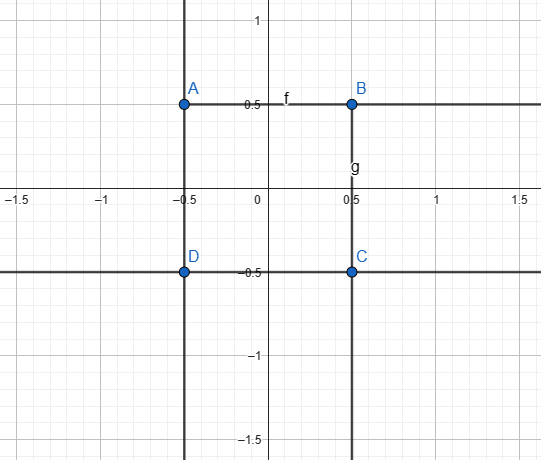
\includegraphics[width = 0.5\textwidth]{image/square_illustrator.png}
\end{figure} \par 
Thực hiện nhiều thí nghiệm với các cặp tham số a, b khác nhau ta được một vài kết luận nhỏ:
% insert multiple images
\begin{figure}[!ht]
  \centering
  \begin{subfigure}[b]{0.3\linewidth}
    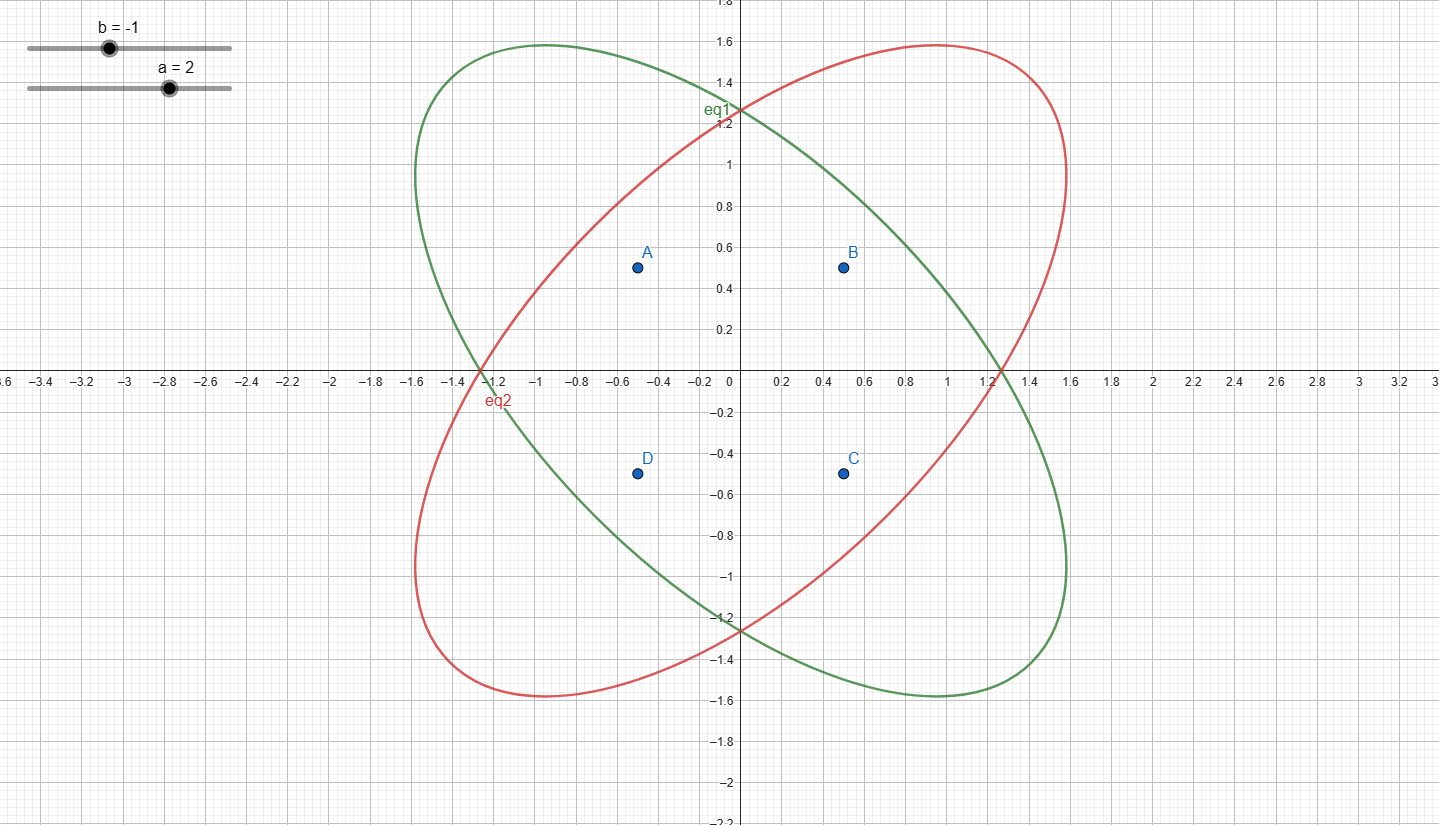
\includegraphics[width=\linewidth]{image/square_illustrator_1.png}
    \caption{a = 2, b = -1}
  \end{subfigure}
  \begin{subfigure}[b]{0.3\linewidth}
    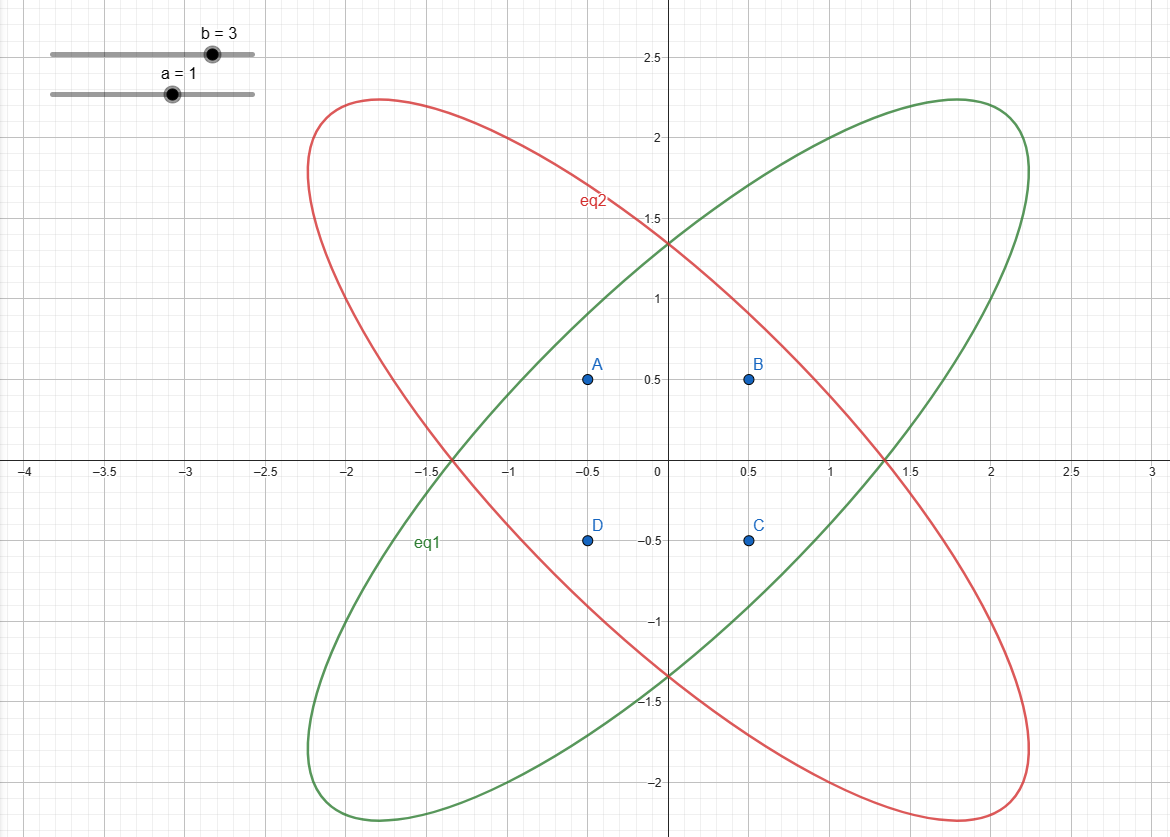
\includegraphics[width=\linewidth]{image/square_illustrator_2.png}
    \caption{a = 1, b = 3}
  \end{subfigure}
  \begin{subfigure}[b]{0.3\linewidth}
    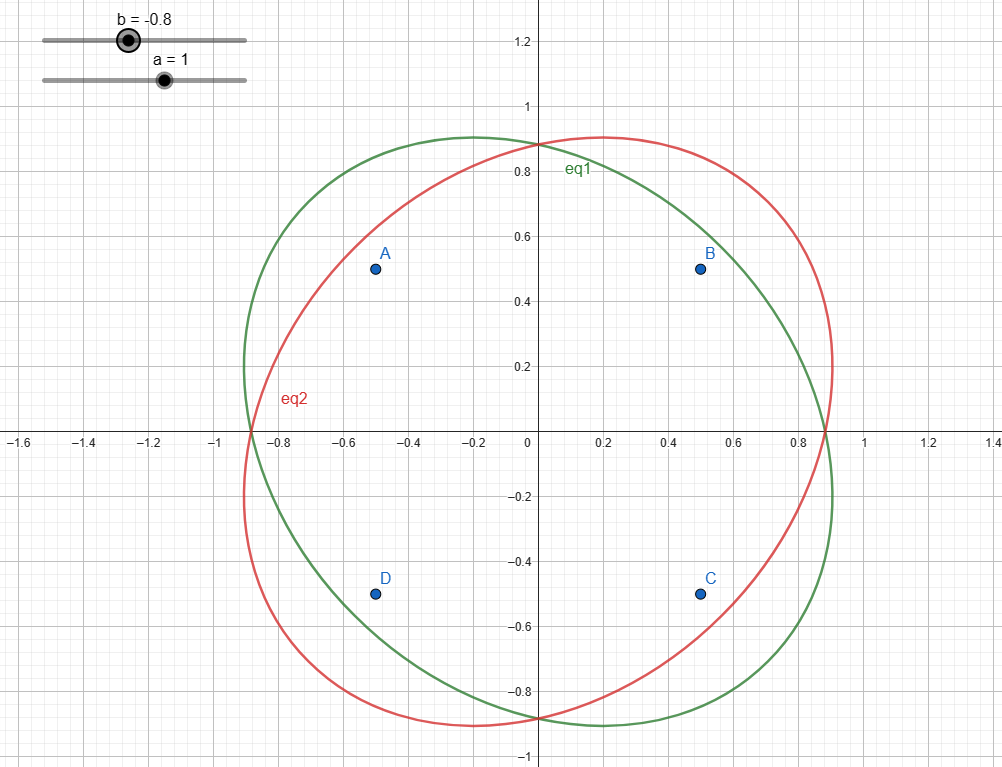
\includegraphics[width=\linewidth]{image/square_illustrator_3.png}
    \caption{a = 1, b = -0.8}
  \end{subfigure}
\end{figure} \par
Tỉ lệ của $\frac{\left\lvert a \right\rvert}{\left\lvert b\right\rvert }$ càng gần 0 thì elip có xu hướng ''nhọn'' hoặc ''dẹt'' về 2 đầu, ngược lại, tỉ lệ càng gần 1 thì elip có xu hướng ''tròn'' hơn. Và thực vậy, khi a = b thì ta được phương trình đường tròn. \par
Như vậy, từ 3 hình trên ta có thê xác định tỉ lệ $\frac{\left\lvert a \right\rvert}{\left\lvert b\right\rvert }$ để được khung hình elip như mong muốn, tỉ lệ này sẽ xấp xỉ 2. Vai trò của a, b có một chút ''đặc biệt'', cụ thể, nếu $\left\lvert a \right\rvert > \left\lvert b \right\rvert$ thì elip đỏ (tượng trưng cho dấu cộng trong phương trình \ref{eq:elip}) nghiêng về bên phải, ngược lại, elip xanh (tượng trưng cho dấu trừ trong phương trình \ref{eq:elip}) nghiêng về bên trái. Để thống nhất hướng nghiêng của elip, ta sẽ chọn a, b sao cho $\left\lvert a \right\rvert < \left\lvert b \right\rvert$. \par
Sau khi tìm được a, b mong muốn, ta cần nhân với side để mở rộng elip phù hợp kích thước ảnh ban đầu.
\paragraph{Mô tả:} Đầu tiên ta tìm toạ độ vị trí trung tâm của hình elip cần cắt. Cách tính đại lượng này tương tự cách tìm tâm hình tròn. Tiếp theo, với 2 giá trị a, b tìm được từ phần ý tưởng, ta tìm được giá trị \textit{new\_a}, \textit{new\_b} tương ứng với kích thước ảnh ban đầu. Sau đó, ta tạo ra 2 mask, mỗi mask là một hình elip, bằng cách sử dụng hàm \textit{numpy.ogrid} và phương trình elip đã được đưa ra. Sau đó, ta gán giá trị 0 cho các điểm ảnh nằm ngoài cả 2 mask. \par
Việc gọi hai biến \textit{const\_1} và \textit{const\_2} là vì ta muốn đơn giản việc tính toán giá trị của $\frac{1}{a^2} + \frac{1}{b^2}$ và $\frac{1}{a^2} - \frac{1}{b^2}$
Áp dụng ý tưởng tìm a, b như phần ý tưởng bên trên cùng mô phỏng trên GeoGebra, ta chọn a = 0.3, b = 0.6 và thu được kết quả như hình bên dưới:
\begin{figure}[!ht]
  \centering
  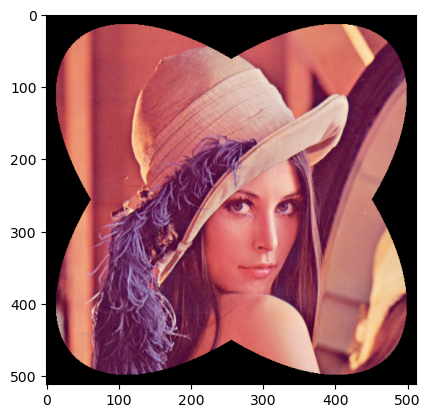
\includegraphics[width=0.5\textwidth]{image/lenna_03_06.png}
\end{figure} \par
Có thể thấy, khung elip được định hình nhưng khung vẫn chưa chạm các cạnh ngoài của bức ảnh. Sử dụng kĩ thuật chặt nhị phân, giá trị a, b tìm được là 0.35 và 0.61375 (với bức ảnh kích thước 1$\times$1), ảnh đầu ra đạt độ chính xác 99.1\% so với bức ảnh đề bài (tham khảo kết quả từ phép đo tại website: \href{https://www.imgonline.com.ua/eng/similarity-percent.php}{imgonline.com.ua}). \par
Việc tạo bản sao của ảnh đầu vào và thay đổi kích thước ảnh đầu ra để phù hợp với kích thước ảnh đầu vào là để tránh việc mảng điểm ảnh truyền vào bị thay đổi, đã được trình bày rõ hơn ở phần cuối mô tả ở hàm \textit{circular\_crop}.
\subsection{Nhóm hàm bổ trợ}
\subsubsection{Hàm limit\_value}
\textbf{Input:} Mảng NumPy 2 chiều các điểm ảnh \textit{img\_2d}. \\
\textbf{Output:} Mảng NumPy 2 chiều các điểm ảnh với các giá trị đã được giới hạn trong khoảng [0, 255].

\paragraph{Ý tưởng thực hiện:} Trong quá trình tính toán giá trị mới cho các phần tử màu trong điểm ảnh, không thể tránh khỏi trường hợp giá trị mới vượt quá khoảng [0, 255]. Vì vậy, ta cần giới hạn giá trị mới trong khoảng [0, 255]. \par
Ta không thể lần lượt thay đổi từng phần tử trong mảng 2 chiều, vì vậy ta thay thế phương pháp thủ công bằng cách gọi hàm \textit{numpy.clip} để giới hạn giá trị của từng phần tử mảng \textit{img\_2d} trong khoảng [0, 255].
\paragraph{Mô tả:} Hàm sử dụng phương thức \textit{numpy.clip} của thư viện NumPy để giới hạn giá trị pixel của hình ảnh đầu vào trong khoảng từ 0 đến 255. Kết quả cuối cùng là một hình ảnh mới với giá trị pixel được giới hạn trong khoảng từ 0 đến 255. Mặc dù mang tên là clip nhưng phương thức này không ''cắt bỏ'' những giá trị không hợp lệ trong khoảng (min, max) mà chỉ đơn giản là thay thế những giá trị nằm ngoài khoảng (min, max) bằng min hoặc max. \par
Sở dĩ có hàm này để giới hạn giá trị nhưng ta vẫn ép kiểu uint8 cho mảng output trong nhóm hàm chính là vì kiểu dữ liệu trả về có thể có kiểu dữ liệu khác. Vì vậy, ta cần ép kiểu về uint8. Và đồng thời, đảm bảo tính ''duy nhất'' của việc lập trình hàm, rằng một hàm chỉ thực hiện một chức năng, ta không nên vừa thực hiện việc giới hạn giá trị và ép kiểu dữ liệu trong một hàm. 
\subsubsection{Hàm show\_image}
\textbf{Input:} Danh sách các ảnh đầu ra ở dạng mảng NumPy 2 chiều các điểm ảnh (\textit{img\_list}) \\
\textbf{Output:} Không có.

\paragraph{Ý tưởng thực hiện:} Xuất phát từ ý tưởng lưu ảnh đầu ra vào một danh sách, ta sẽ duyệt qua từng ảnh trong danh sách và hiển thị ảnh đó ra màn hình. Để có thể hiển thị nhiều ảnh trên một figure, ta sử dụng phương thức \textit{subplot} của thư viện Matplotlib. Danh sách này luôn chứa ảnh đầu tiên (phần tử đầu tiên) là ảnh gốc, tuỳ thuộc vào chức năng mà người dùng nhập vào chương trình khi khởi chạy, danh sách này có thể có 2, 3 hoặc 12 ảnh. Ứng với từng trường hợp mà cách sắp xếp các subplot trên figure sẽ khác nhau.  

\paragraph{Mô tả:} Để có thể hiển thị nhiều ảnh trên một figure, ta sử dụng phương thức \textit{subplot}. Xét đến toàn bộ các trường hợp có thể xảy ra khi hàm \textit{main} được khởi chạy, sẽ chỉ có các trường hợp có 2, 3, 12 ảnh được in ra. Do đó, ta xét cụ thể từng trường hợp và nhận thấy rằng với hai trường hợp đầu, ảnh có thể được hiển thị thành một hàng, còn với trường hợp cuối, ảnh có thể được hiển thị thành 3 hàng. Trong phương thức \textit{subplot}, với hai trường hợp đầu, ta truyền số hàng (nrows) là 1 và số cột (ncols) là kích thước của danh sách ảnh đầu ra (\textit{len(img\_list)}), còn với trường hợp cuối, ta truyền số hàng là 3 và số cột là 4. Và dù là trường hợp nào thì thành phần cuối cùng của tham số - chỉ số - đều là chỉ số của ảnh trong danh sách ảnh đầu ra. \par

Dòng code \textit{plt.figure(figsize=(20,15))} có tác dụng tạo figure hiển thị ra màn hình với kích thước 20x15 inches thay vì thông số mặc định 6.4x4.8 nhằm đảm bảo tính thẩm mỹ, không có tác động đến kết quả xử lý.

\subsubsection{Hàm write\_image}
\textbf{Input:} Danh sách các ảnh đầu ra ở dạng mảng NumPy 2 chiều các điểm ảnh (\textit{img\_list}), danh sách tên các ảnh đầu ra (\textit{img\_name\_list}) \\
\textbf{Output:} Không có.
\paragraph{Ý tưởng thực hiện:} Với yêu cầu đề bài lưu ảnh đầu ra tương ứng với từng chức năng, ta cần lưu tên hoặc ít nhất hậu tố chức năng của ảnh đầu ra ứng với từng hàm chức năng, và để có thể thuận tiện cho việc lưu trữ cũng như truy xuất, ta sử dụng kiểu dữ liệu \textit{list} để lưu tên ảnh đầu ra. Kết hợp với phương thức \textit{imsave} của thư viện Matplotlib, ta sẽ lần lượt lưu từng ảnh trong danh sách ảnh đầu ra với tên tương ứng.
\paragraph{Mô tả:} Với ý tưởng được nêu trên, việc sử dụng list comprehension sẽ giúp ta viết code ngắn gọn hơn. Tuy nhiên, ta sẽ bắt đầu thực hiện động tác lưu ảnh từ phần tử thứ hai (chỉ số bằng 1) để tránh can thiệp vào ảnh gốc (phần tử đầu tiên).

\subsubsection{Hàm main}
\textbf{Input:} Không có. \\
\textbf{Output:} Không có.
\paragraph{Ý tưởng thực hiện:} Đóng vai trò là hàm chính của chương trình, hàm \textit{main} sẽ gọi lần lượt các hàm chức năng và hiển thị ảnh đầu ra tương ứng với từng hàm chức năng. Khi được khởi chạy, sẽ có dòng thông báo thể hiện danh sách các chức năng xử lý ảnh, đồng thời cho phép người dùng nhập vào đường dẫn ảnh (trực tiếp hoặc gián tiếp) và chức năng thực hiện. Đồng thời để các hàm thành phần có thể hoạt động theo một trình tự, ta cần lưu tên cũng như hậu tố của bức ảnh đầu vào để đảm bảo ảnh đầu ra thoả yêu cầu đề bài (có cùng tên và đuôi ảnh với ảnh gốc). Về xử lý với từng chức năng người dùng nhập vào, do ngôn ngữ Python chuẩn các phiên bản cũ (3.10 trở về trước), ta sử dụng cấu trúc \textit{if-elif-else} để xử lý. \par
List kết quả không là output của hàm nhưng sẽ xử lý theo hướng list các tuple với phần tử đầu tiên là mảng NumPy 2 chiều các điểm ảnh, phần tử thứ hai là tên ảnh đầu ra tương ứng với hàm chức năng. Để có thể hiển thị ảnh đầu ra, ta sử dụng hàm \textit{write\_image} để lưu ảnh đầu ra và hiển thị ảnh đầu ra tương ứng với hàm chức năng. Đồng thời, ta cũng sử dụng hàm \textit{show\_image} để hiển thị ảnh. \par
\paragraph{Mô tả:} Đầu tiên, hàm in ra các chức năng xử lý ảnh, sau đó yêu cầu người dùng nhập vào đường dẫn ảnh đầu vào và chức năng xử lý ảnh. Nếu đường dẫn ảnh và chức năng hợp lệ, ta sẽ lưu tên ảnh đầu vào và hậu tố ảnh đầu vào. Tuỳ thuộc vào chức năng được gọi mà (các) hàm chức năng tương ứng sẽ được thực thi và kết quả thu được sẽ được thêm vào danh sách \textit{result} (list các tuple). \par
Với các chức năng chỉ 1 tuple trả về, ta dùng phương thức \textit{append} quen thuộc, tuy nhiên, để tránh việc lặp code, với những chức năng trả về từ 2 tuple (ví dụ lật ảnh ngang/dọc trả về cùng lúc ảnh lật ngang và ảnh lật dọc mà không cần hỏi người dùng) ta sử dụng phương thức \textit{extend} để thêm các tuple vào danh sách. Phương thức extend cho phép thêm liên tiếp các phần tử của một vào một list khác. Sau khi thực hiện xong các hàm chức năng, ta sẽ lưu ảnh đầu ra và hiển thị ảnh đầu ra tương ứng với hàm chức năng. \par
Khi xét đến kết quả trả về của các hàm chức năng, ta không truyền vào tên ảnh đầu vào là một tham số nên để phân biệt tên giữa các hàm, ta sẽ lưu thêm hậu tố vào tên ảnh đầu ra. Kết quả đó được thêm vào list \textit{result} và trước khi gọi hàm \textit{write\_image}, ta còn chỉnh sửa lại tên của bức ảnh đầu ra bằng việc cộng chuỗi. Đồng thời list trên cũng được phân rã (parse) lấy phần tử đầu tiên thêm vào list \textit{img\_list} để hiển thị ảnh đầu ra và phần tử thứ hai (sau khi xử lý chuỗi) thêm vào list \textit{img\_list\_name} để lưu tên ảnh đầu ra và gọi hàm \textit{show\_image} cũng như \textit{write\_image}.

\subsection{Hình ảnh đầu ra ứng với từng chức năng}
\begin{figure}[!ht]
  \centering
  \begin{subfigure}[b]{0.45\linewidth}
    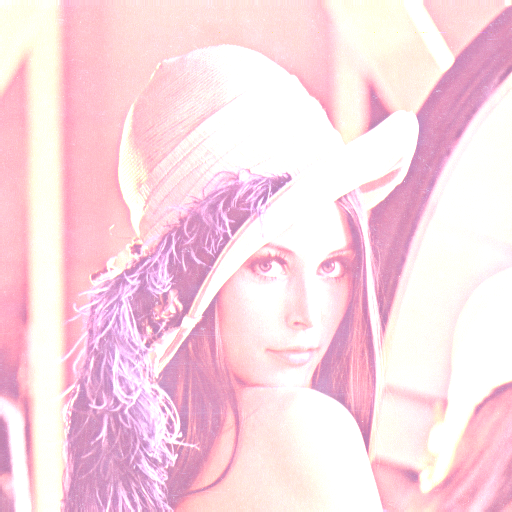
\includegraphics[width=\linewidth]{image/Lenna_brightness_128.png}
    \caption{Thay đổi độ sáng (brightness=128)}
  \end{subfigure}
  \begin{subfigure}[b]{0.45\linewidth}
    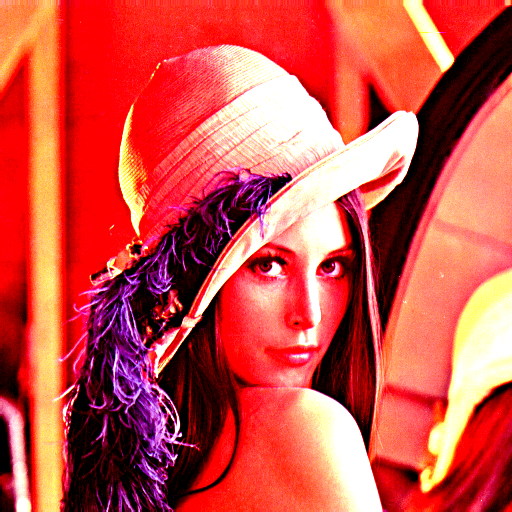
\includegraphics[width=\linewidth]{image/Lenna_contrast_128.png}
    \caption{Thay đổi độ tương phản (contrast=128)}
  \end{subfigure}
\end{figure}
\pagebreak

\begin{figure}[!ht]
  \begin{subfigure}[b]{0.45\linewidth}
    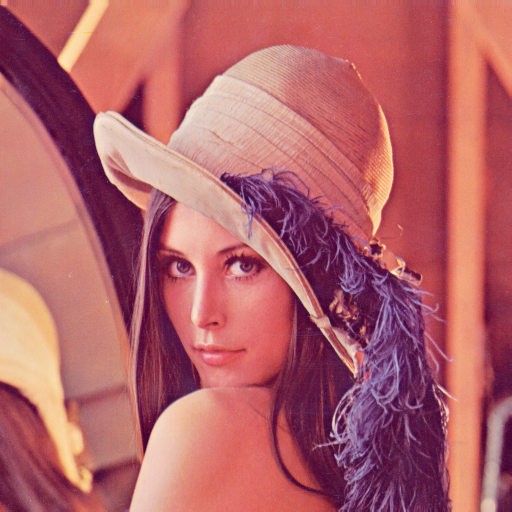
\includegraphics[width=\linewidth]{image/Lenna_flip_horizontal.png}
    \caption{Lật ảnh ngang}
  \end{subfigure}
  \begin{subfigure}[b]{0.45\linewidth}
    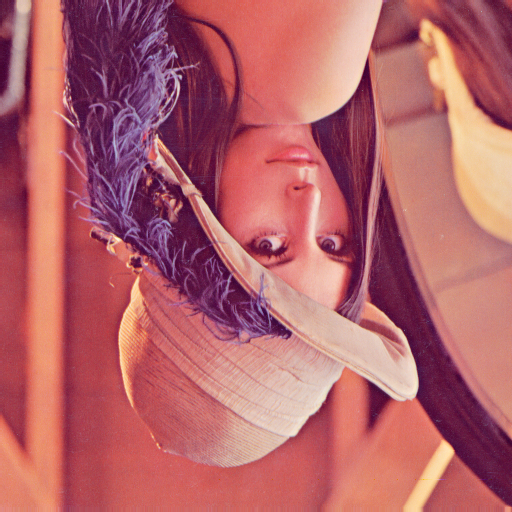
\includegraphics[width=\linewidth]{image/Lenna_flip_vertical.png}
    \caption{Lật ảnh dọc}
  \end{subfigure}
\end{figure}
\pagebreak
\begin{figure}[!ht]
  \begin{subfigure}[b]{0.45\linewidth}
    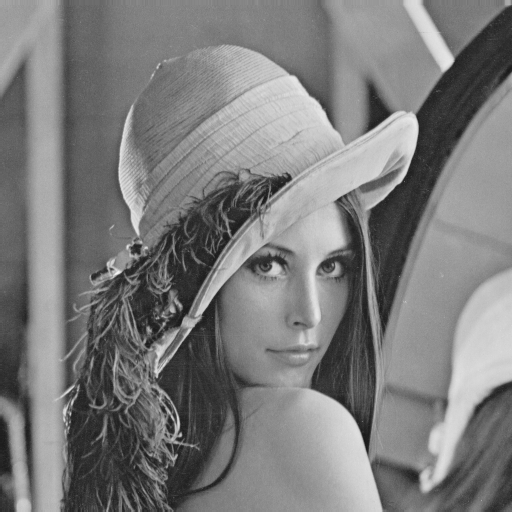
\includegraphics[width=\linewidth]{image/Lenna_grayscale.png}
    \caption{Chuyển sang ảnh xám}
  \end{subfigure}
  \begin{subfigure}[b]{0.45\linewidth}
    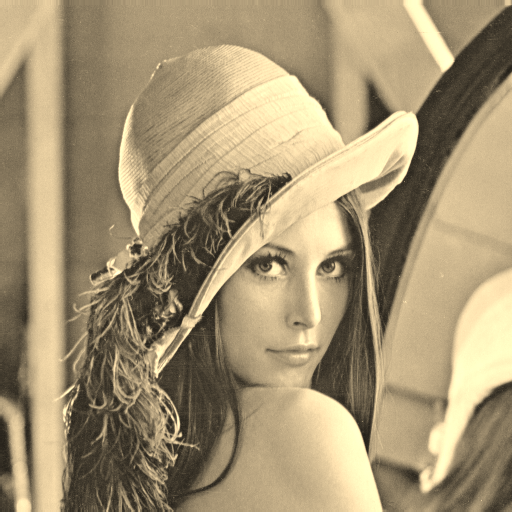
\includegraphics[width=\linewidth]{image/Lenna_sepia.png}
    \caption{Chuyển sang ảnh Sepia}
  \end{subfigure}
\end{figure}

\begin{figure}[!ht]
  \begin{subfigure}[b]{0.45\linewidth}
    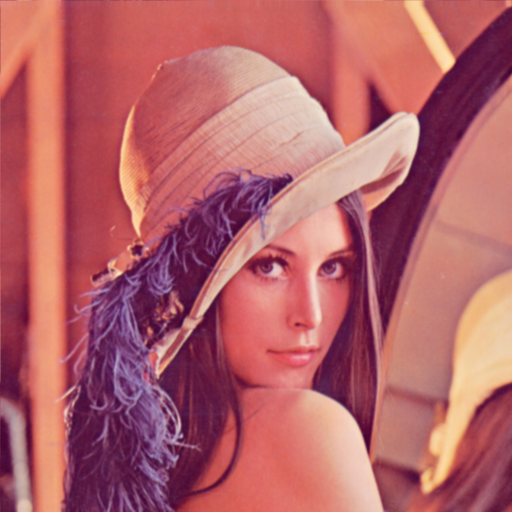
\includegraphics[width=\linewidth]{image/Lenna_blur.png}
    \caption{Làm mờ ảnh với kernel size = 3}
  \end{subfigure}
  \begin{subfigure}[b]{0.45\linewidth}
    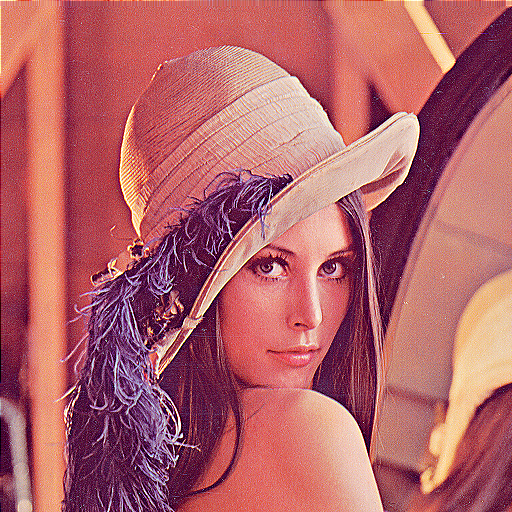
\includegraphics[width=\linewidth]{image/Lenna_sharpen.png}
    \caption{Làm sắc nét ảnh}
  \end{subfigure}
\end{figure}

\begin{figure}[!ht]
  \begin{subfigure}[b]{0.3\linewidth}
    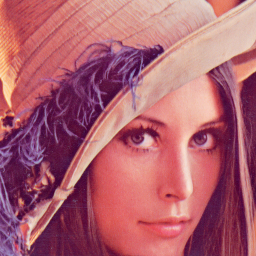
\includegraphics[width=\linewidth]{image/Lenna_center_crop.png}
    \caption{Cắt ảnh tại tâm với kích thước 256x256}
  \end{subfigure}
  \begin{subfigure}[b]{0.3\linewidth}
    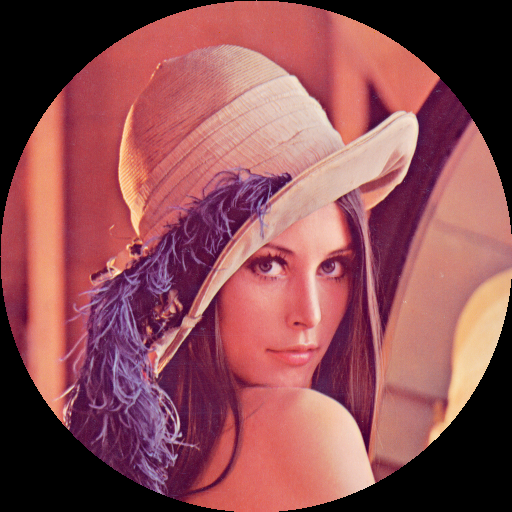
\includegraphics[width=\linewidth]{image/Lenna_circular_crop.png}
    \caption{Cắt ảnh theo khung hình tròn}
  \end{subfigure}
  \begin{subfigure}[b]{0.3\linewidth}
    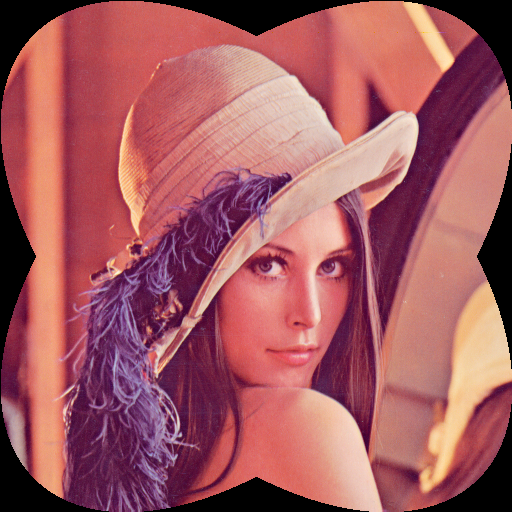
\includegraphics[width=\linewidth]{image/Lenna_elliptical_crop.png}
    \caption{Cắt ảnh theo khung hình elip}
  \end{subfigure}
\end{figure}
\newpage

\section{Tài liệu tham khảo}
\begin{itemize}
  \item Brightness
  \begin{enumerate}
    \item \href{https://ie.nitk.ac.in/blog/2020/01/19/algorithms-for-adjusting-brightness-and-contrast-of-an-image/}{Algorithms for adjusting brightness and contrast of an image}
  \end{enumerate}
  \item Contrast
  \begin{enumerate}
      \item \href{https://www.dfstudios.co.uk/articles/programming/image-programming-algorithms/image-processing-algorithms-part-5-contrast-adjustment/}{Image Processing Algorithms Part 5 - Contrast Adjustment}
  \end{enumerate}
  \item Flip
  \begin{enumerate}
      \item \href{https://www.w3schools.com/python/numpy/numpy_array_slicing.asp}{NumPy Array Slicing}
  \end{enumerate}
  \item Grayscale/Sepia Conversion
  \begin{enumerate}
    \item \href{https://www.tutorialspoint.com/dip/grayscale_to_rgb_conversion.htm}{Convert RGB to Grayscale}
    \item \href{https://www.geeksforgeeks.org/image-processing-in-java-colored-image-to-sepia-image-conversion/}{Convert RGB to Sepia}
    \item \href{https://numpy.org/doc/stable/reference/generated/numpy.dot.html}{NumPy dot}
    \item \href{https://numpy.org/doc/stable/reference/generated/numpy.repeat.html}{NumPy repeat}
  \end{enumerate}
  \item Convolute 2D
  \begin{enumerate}
    \item \href{https://en.wikipedia.org/wiki/Kernel\_(image\_processing)}{Kernel (image processing)}
    \item \href{https://en.wikipedia.org/wiki/File:2D_Convolution_Animation.gif}{2D Convolution Animation}
    \item \href{https://en.wikipedia.org/wiki/Convolution#Discrete_convolution}{Discrete convolution}
    \item \href{https://en.wikipedia.org/wiki/Fast_Fourier_transform}{Fast Fourier transform}
    \item \href{https://numpy.org/doc/stable/reference/generated/numpy.fft.fftn.html}{NumPy fftn}
    \item \href{https://codeforces.com/blog/entry/43499}{FFT and Convolution - Codeforces}
    \item \href{https://numpy.org/doc/stable/reference/generated/numpy.fft.ifftn.html#numpy.fft.ifftn}{NumPy ifftn}
    \item \href{https://numpy.org/doc/stable/reference/generated/numpy.pad.html}{NumPy pad}
  \end{enumerate}
  \item Blur (Gaussian Blur) / Sharpen (Unsharp Mask) image
  \begin{enumerate}
    \item \href{https://en.wikipedia.org/wiki/Kernel\_(image\_processing)}{Kernel (image processing)}
  \end{enumerate}
  \item Circular crop
  \begin{enumerate}
    \item \href{https://numpy.org/doc/stable/reference/generated/numpy.ogrid.html}{NumPy ogrid}
  \end{enumerate}
  \item Elliptical crop
  \begin{enumerate}
    \item \href{https://math.stackexchange.com/questions/426150/what-is-the-general-equation-of-the-ellipse-that-is-not-in-the-origin-and-rotate}{Rotate ellipse}
    \item \href{https://www.maa.org/external_archive/joma/Volume8/Kalman/General.html}{General equation of ellipse}
    \item \href{https://geogebra.org/graphing}{GeoGebra}
  \end{enumerate}
  \item Limit value
  \begin{enumerate}
    \item \href{https://numpy.org/doc/stable/reference/generated/numpy.clip.html}{NumPy clip}
  \end{enumerate}
  \item Show image
  \begin{enumerate}
    \item \href{https://matplotlib.org/stable/api/_as_gen/matplotlib.pyplot.subplot.html}{Matplotlib subplot}
  \end{enumerate}
  \item Write image
  \begin{enumerate}
    \item \href{https://matplotlib.org/stable/api/_as_gen/matplotlib.pyplot.imsave.html}{Matplotlib imsave}
  \end{enumerate}
  \item Main
  \begin{enumerate}
    \item \href{https://www.freecodecamp.org/news/python-switch-statement-switch-case-example/}{Switch case in Python}
    \item \href{https://www.w3schools.com/python/ref_list_extend.asp}{List extend}
  \end{enumerate}
\end{itemize}
 
\end{document}